Lorsqu'on utilise l'implicit tiling, le client Cesium à besoin de recevoir en premier lieu une liste de tuiles disponibles. Cette liste doit lui être donnée sous forme de Subtree. Les \textit{Subtrees} dans Cesium constituent une composante essentielle pour la gestion et l'optimisation de la visualisation des données géospatiales volumineuses. Plutôt que de charger l'intégralité des données géospatiales, les Subtrees ont pour but d'indiquer au client Cesium quelles tuiles sont disponibles, quelles tuiles ont un contenu à afficher quelles sont ses enfants (\texttt{children}). Pour chacune de ces trois informations, un Subtree contient un objet \textit{Availability} (\autoref{sec:availability-class}) stockant une liste de boolean représentant chaque tuile. Pour savoir quel index de cette liste correspond à quelle tuile, un autre style de \textit{Binary Space Partitioning} est utilisé. Une \href{https://en.wikipedia.org/wiki/Z-order\_curve}{\textit{Z-order curve} ou un \textit{Morton order}}\footnote{https://en.wikipedia.org/wiki/Z-order\_curve} est utilisé pour définir les indexes (\autoref{sec:morton}).

Une fois ces Subtrees générés, il faudra les envoyer au client. Cela se fera en les transformant en JSON puis en un fichier respectant le \href{https://github.com/CesiumGS/3d-tiles/tree/main/specification/ImplicitTiling\#subtree-binary-format}{\textit{Subtree Binary Format}}\footnote{https://github.com/CesiumGS/3d-tiles/tree/main/specification/ImplicitTiling\#subtree-binary-format}

\subsection*{Hiérarchie de Subtrees}

\begin{figure}[H]
    \centering
    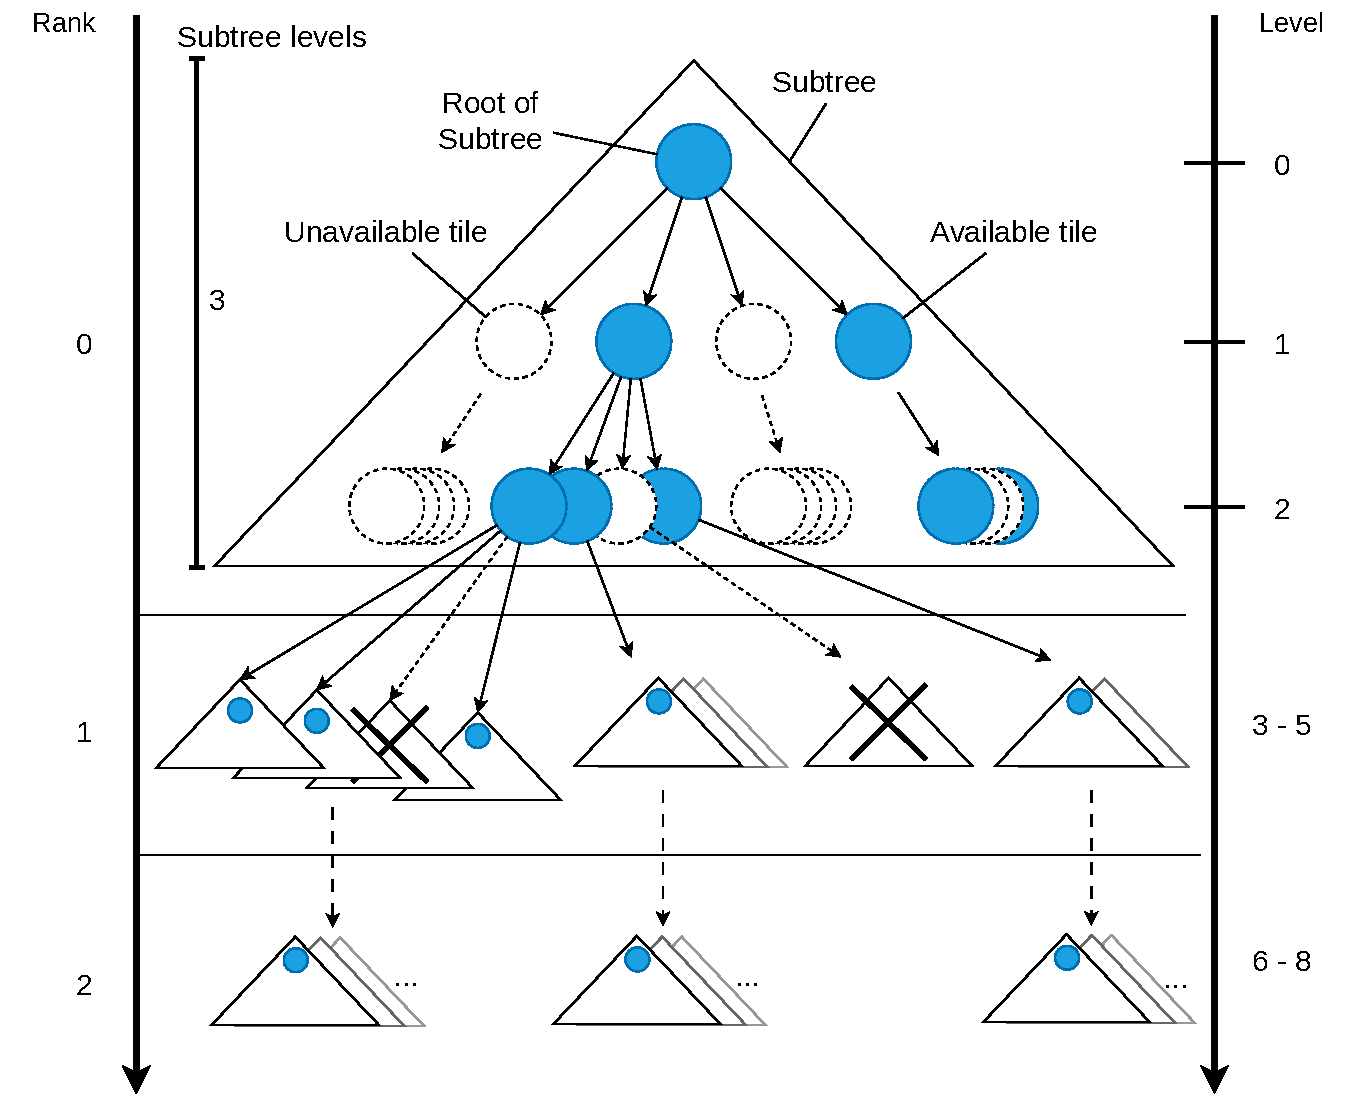
\includegraphics[width=1\textwidth]{assets/figures/Subtree_hierarchy.drawio.pdf}
    \caption{Exemple de hiérarchie de Subtrees}
    \label{fig:subtree-hierarchy}
\end{figure}

Le Tileset est partitionné en Subtrees de taille \texttt{subtreeLevels} fixe. Leur schéma de subdivision suit la même logique que les tuiles d'un implicit tiling. Chaque \textit{level} ou niveau représente une subdivision de la tuile de niveau inférieur. Un Subtree est généralement composé de plusieurs niveau de profondeur. Chaque niveau est composé d'une liste de noeuds représentant la disponibilité d'une tuile. En fonction du schema de subdivision, quadtree ou octree, chaque noeuds peut avoir 4 ou 8 enfants respectivement. On peut retrouver ces noeuds dans les listes de disponibilités citées plus haut. Les \textit{Availabilities} seront traités plus en détails dans la section \ref{sec:availability-class}.

Plusieurs Subtrees peuvent être liés entre eux pour former un arbre de Subtrees. Leur liaison se fait entre le noeuds \textit{root} d'un subtree et un noeuds au niveau maximum d'un autre Subtree. Par soucis de compréhension, j'appellerai le \textit{rang}, ou \textit{rank} en Anglais, d'un Subtree le niveau de profondeur de ce Subtree par rapport à la racine du Tileset. Le Subtree de rang 0 est le Subtree de la racine du Tileset. Les Subtree de rang maximum sont les Subtrees qui contiendront les contenus à afficher.

Finalement, quelques règles doivent être respectées lors d'une construction d'une hiérarchie de Subtrees:

\begin{itemize}
    \item Les Subtrees doivent être de même taille.
    \item Les Subtrees doivent avoir le même schéma de subdivision.
    \item Un Subtree doit contenir au minimum un niveau.
\end{itemize}

\newpage
\subsection*{Utilité des Subtrees}

Comme dit précédemment, les Subtrees sont utilisés pour indiquer au client Cesium quelles tuiles sont disponibles, quelles tuiles ont un contenu à afficher et quelles sont ses enfants. Ainsi, ils réduisent la quantité de données que le client Cesium demandera à l'API.

Dans la figure \ref{fig:subtree-debug} ci-dessous, vous pouvez observer le partitionnement binaire de l'espace grâce aux lignes de debug de l'application Cesium. Ces lignes suivent le partitionnement binaire que le client Cesium déduit des Subtrees qu'il à reçu. Là où se trouve des bâtiments, l'espace est plus subdivisé.

\begin{figure}[H]
    \centering
    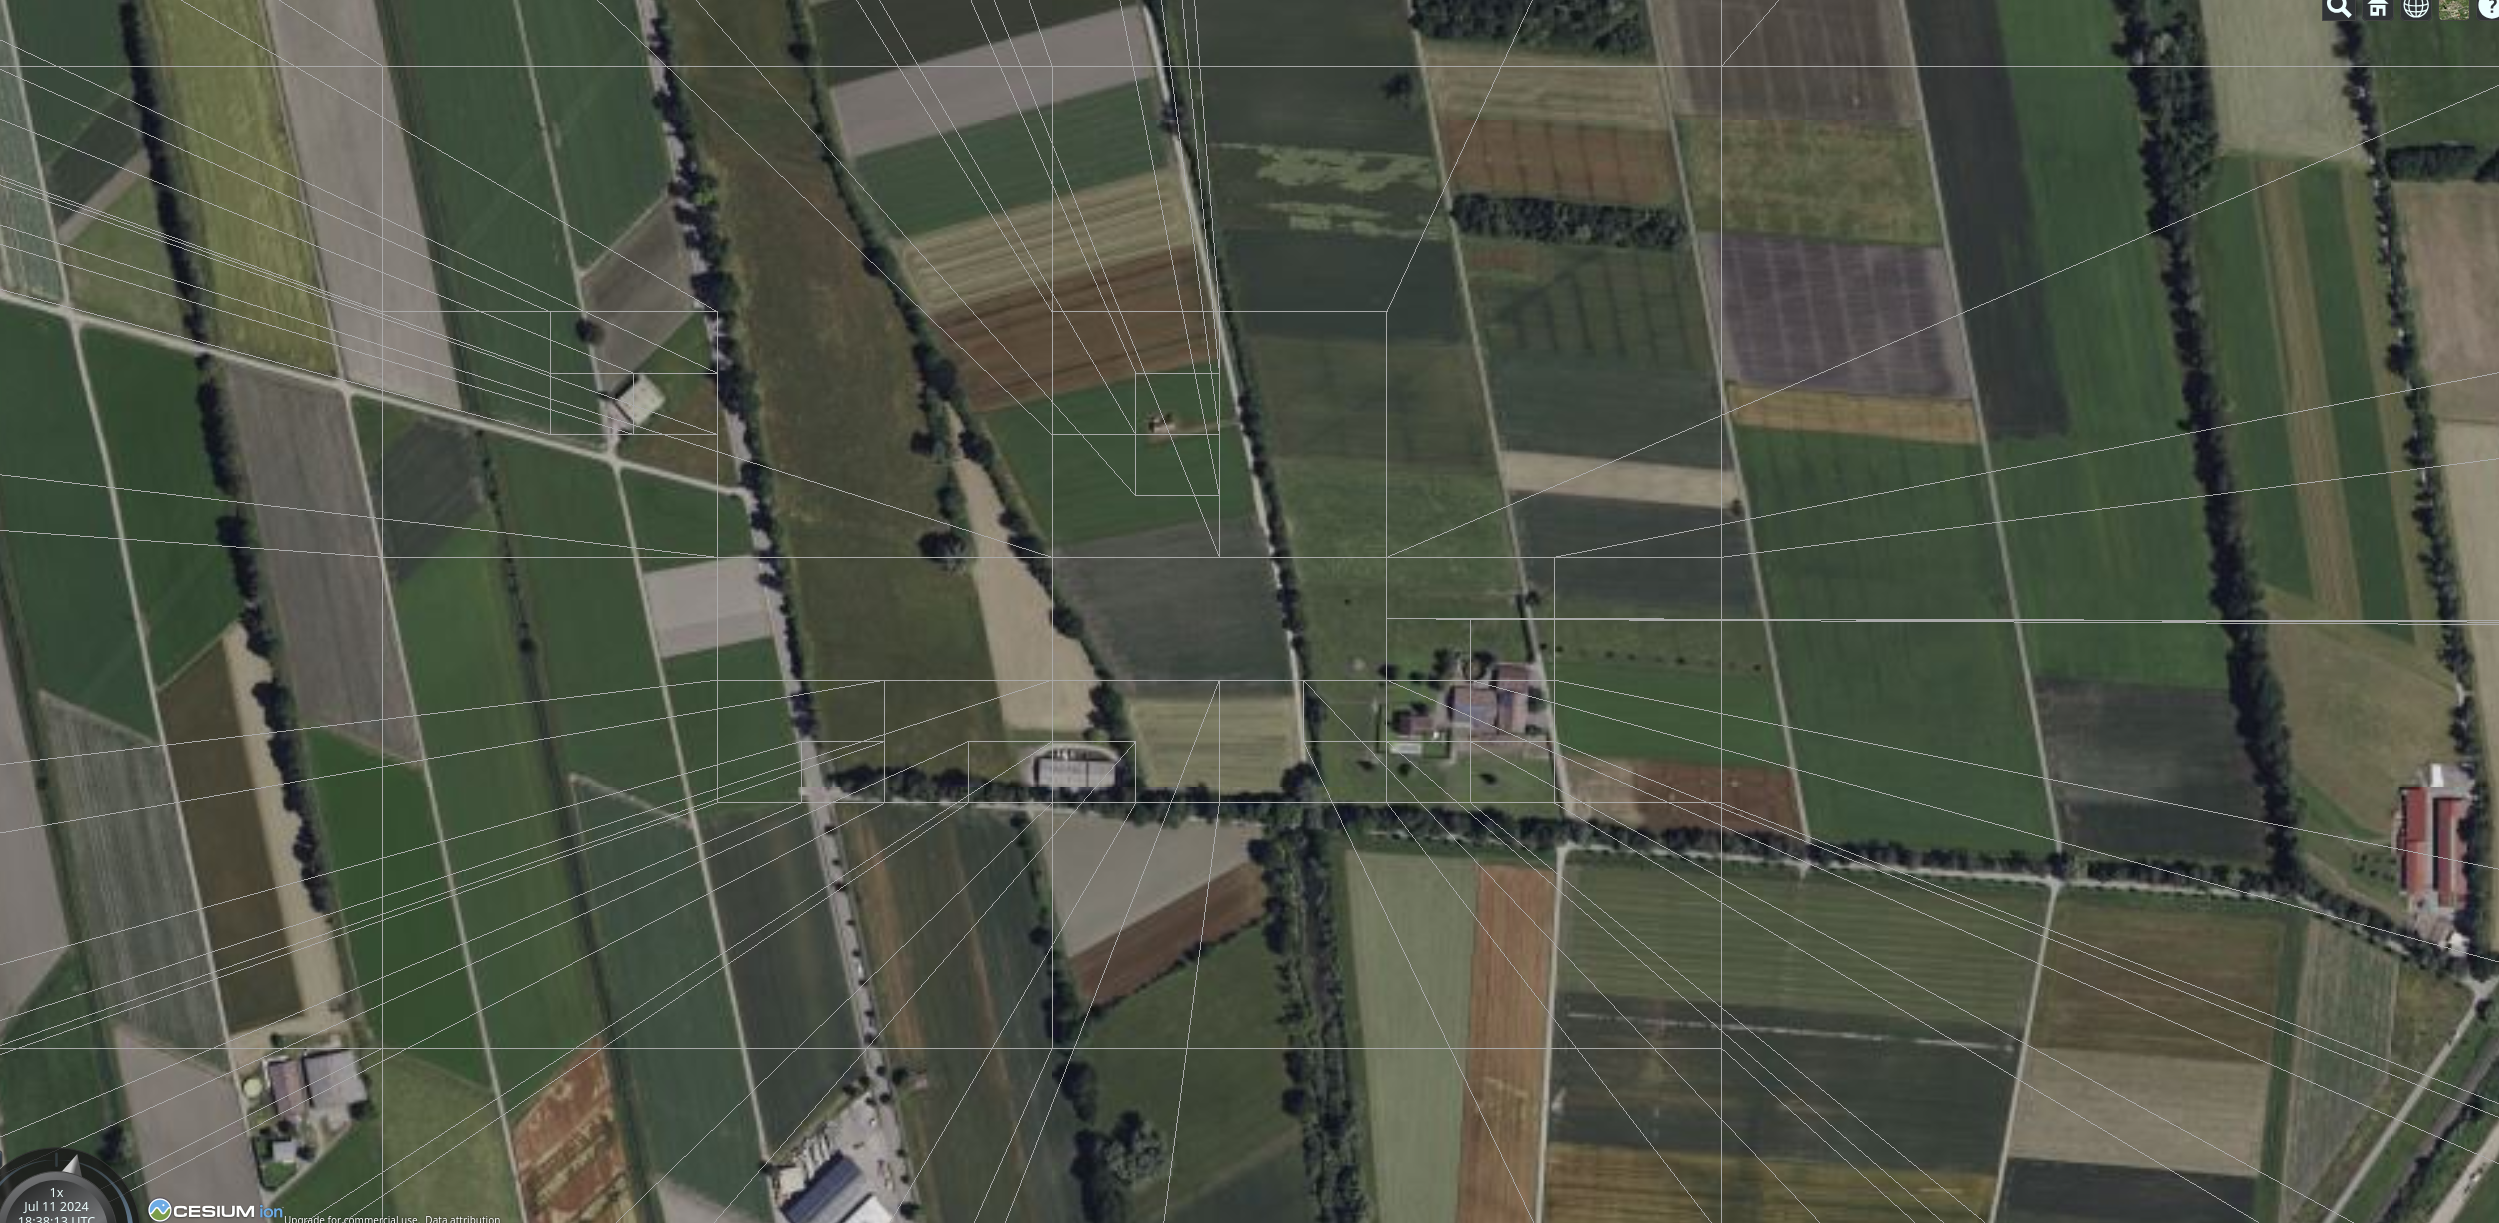
\includegraphics[width=1\textwidth]{assets/figures/Subtree_debug.png}
    \caption{Partitionnement binaire de l'espace}
    \label{fig:subtree-debug}
\end{figure}

Pour comprendre ce que cela signifie, je fais une parallèle avec la section \ref{sec:lod} où j'ai mentionné les niveaux de détails. Il faut comprendre que chacun de ces subdivision est une tuile. Plus une tuile est subdivisée, plus elle elle correspond à un niveau bas dans la hiérarchies du tuilage, plus son contenu est détaillé. J'ai mentionné auparavant que ces niveaux de détails sont définis par la valeur \texttt{geometricError} d'une tuile. c'est toujours le cas. Le client Cesium suit une procédure très simple :

\begin{itemize}
    \item Le client charge une tuile disponible.
    \item Le client calcule le \texttt{Screen Space Error} (SSE) de cette tuile.
    \item Si le seuil SSE est dépassé et que les tuiles enfant sont disponibles, le client charge les tuiles enfant.
\end{itemize}

Ainsi, les tuiles sont chargées en fonction de leur disponibilité fournie par les Subtrees ainsi que leur \texttt{geometricError} et leur distance à la caméra.

\newpage
Un détail très important avec mon implémentation est que les niveaux des Subtrees et des listes de disponibilités sont complètement paramétrables. Actuellement, une seule restriction s'applique :  le contenu affichable ne peut se trouver que dans les Subtree de rang maximal (cf. \autoref{fig:subtree-hierarchy}). J'ai initialement rajouté cette restriction pour forcer l'utilisateur des fonction à garder une structure de la hiérarchie des Subtrees simple, néanmoins elle peut être facilement enlevée si voulu. Pour revenir à la paramétrisation des niveaux des Subtrees, il est possible de définir combien de niveaux contient un Subtree ainsi que le nombre de niveaux le tuilage entier comporte. Ces valeurs doivent être modifiées dans les fichiers :

\texttt{src/main/java/org/apache/baremaps/server/TdTilesResources.java}

et

\texttt{src/main/resources/tdtiles/tileset.json}

Parmi les autres paramètres modifiables, on trouve la possibilité de définir à partir de quels niveaux les tuiles contiennent un certain niveau de détails.

Il est donc possible d'alterner entre une subdivision ayant énormément de niveaux où le contenu ne s'affiche que pour de toutes petites tuiles et une subdivision ayant peu de niveaux où le contenu s'affiche pour des tuiles plus grandes. Cela permet de s'adapter aux tailles de scènes à afficher.